\chapter{Data model}\label{Chap:DataModel}
\begin{figure}[!htb]
   \centering
   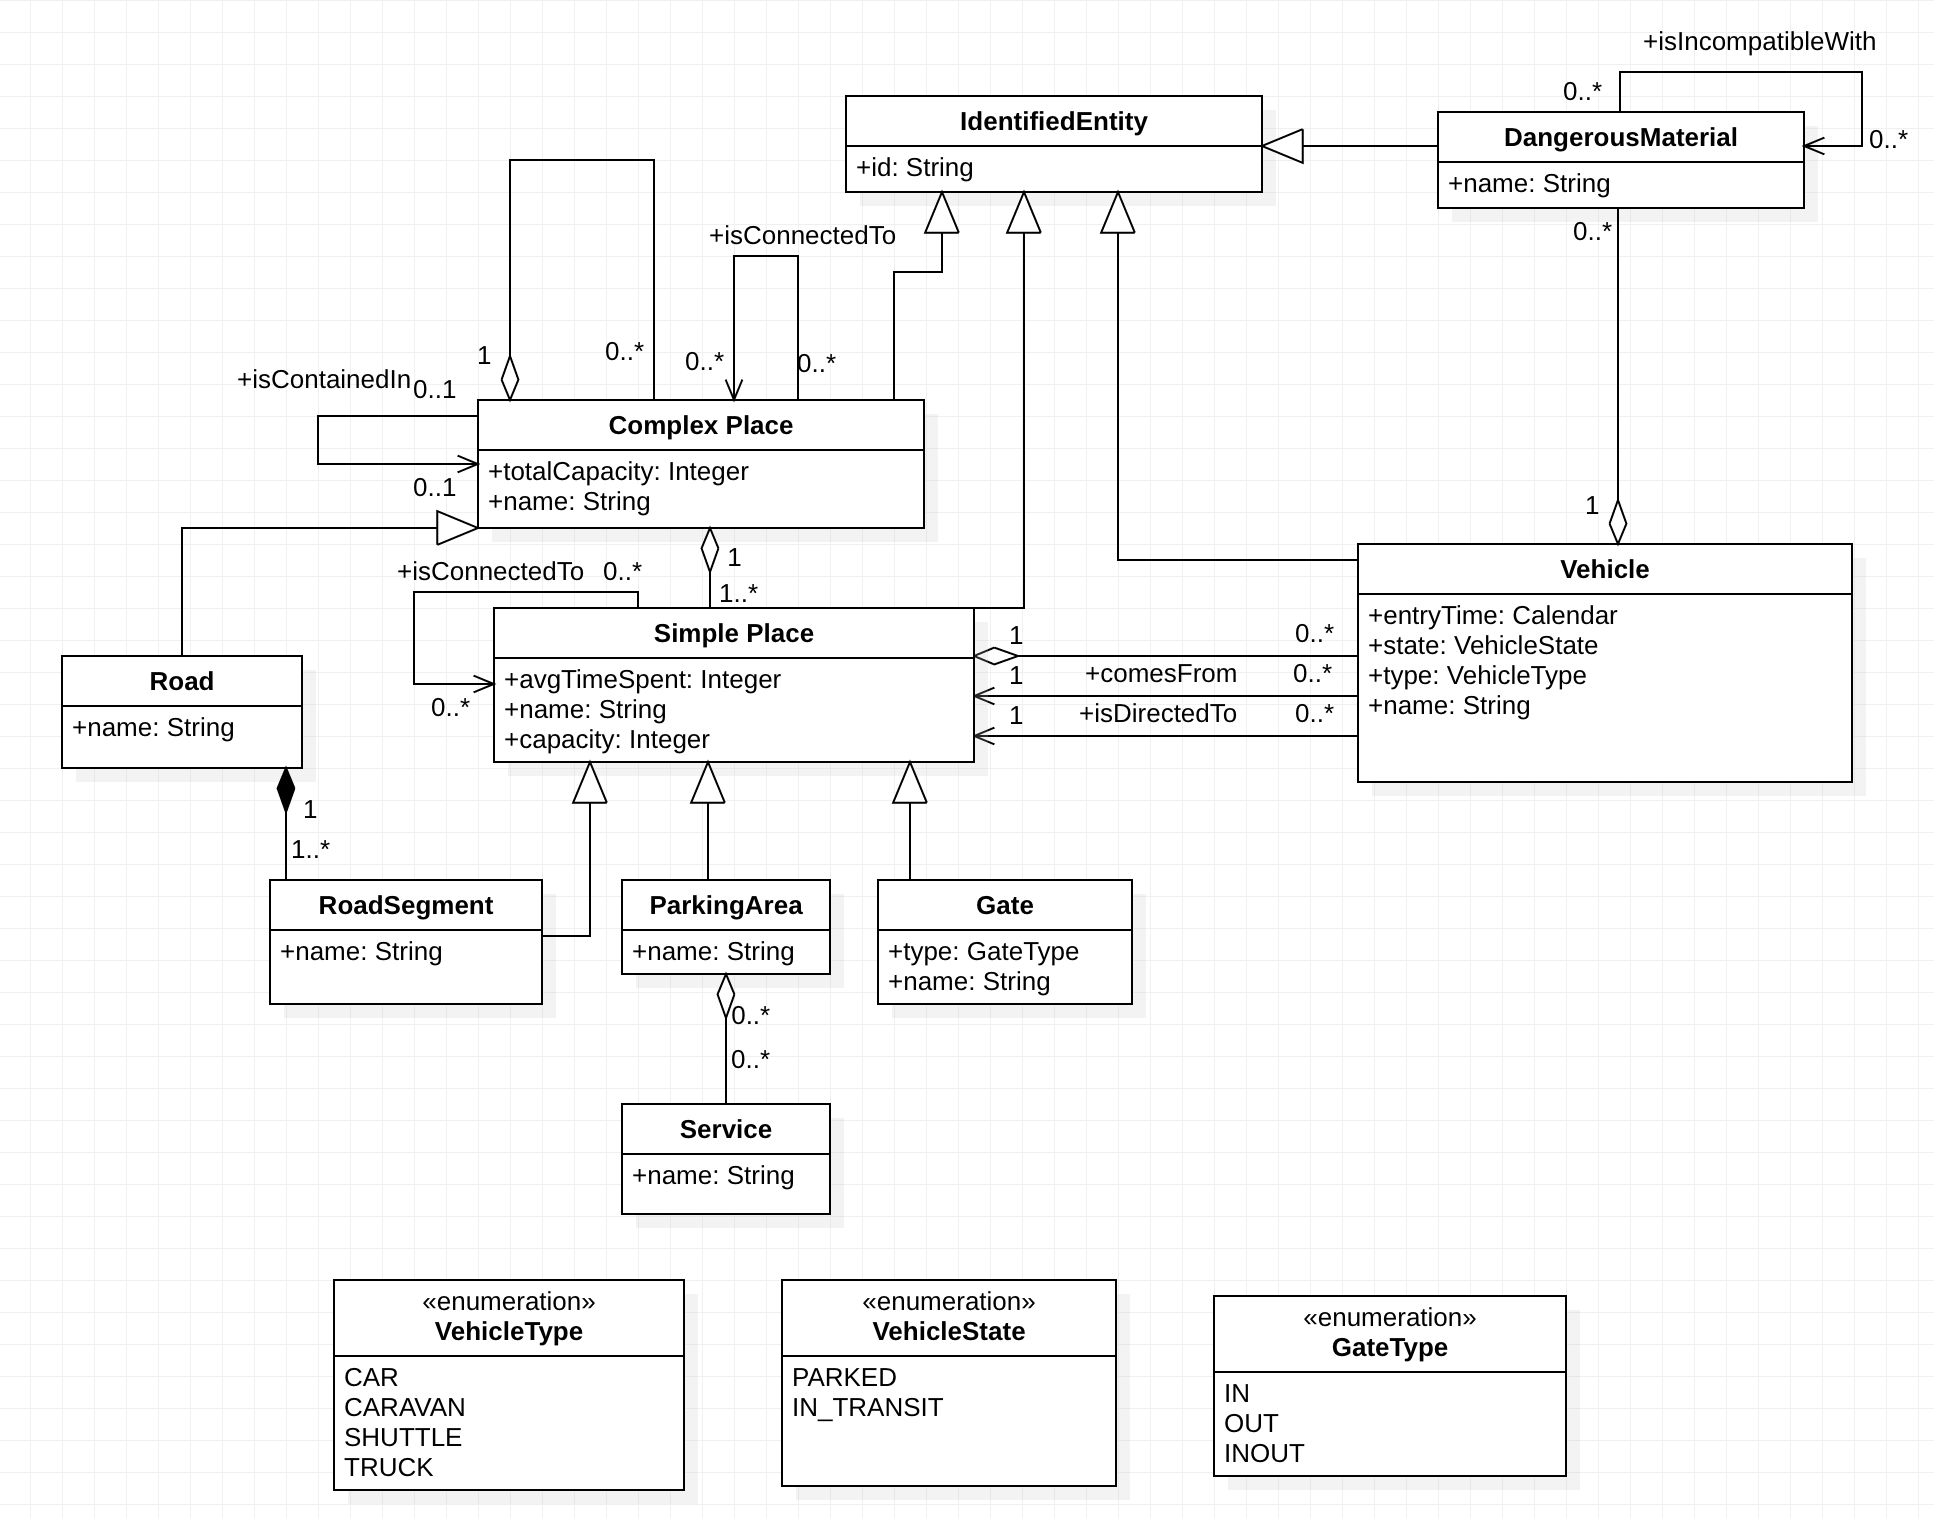
\includegraphics[width=\textwidth]{data_model.png}
   \caption{Data model for the application.}\label{Fig:data_model}
\end{figure}
In figure \ref{Fig:data_model} it is represented the UML model that describes the data handles by the application. Each node of the map can be described as a simple place. Each place has a maximum capacity, that represents the maximum number of vehicle allowed to be in the same time in that place. This property of the places will be exploited as constraint during the evaluation of a path for the entering vehicles. A particularity of this model is the presence of complex places. They have been defined in such way that they can contain a set of simple places or other complex places. For this particular project has been defined only one type of complex place, but if, for future purposes, will be necessary to add other particular complex places, it will be possible to extends the ComplexPlace type.\\
All the information regarding the schema representing the model, are represented in the file \textit{/RNSService/rns/WebContent/WEB-INF/classes/xsd}. The Java classes used in the server application are generated from this file using JAXB.
